\chapter{Conceituação e Idéia Geral}
\label{cha: Conceituação e Idéia Geral}

As seções seguintes descrevem alguns conceitos importantes para que se possa compreender melhor o tema desta monografia. A seção  \ref{sec: Aplicações web escaláveis} descreve o que são aplicações web escaláveis, a \ref{sec:Programação orientada a eventos} programação orientada a eventos, a \ref{sec: Javascript} Javascript e a  \ref{sec: NoSQL - Not Only SQL} NoSQL.


\section{Aplicações web escaláveis}
\label{sec: Aplicações web escaláveis}
\begin{description}
\item[Escalabilidade] \hfill \\
Cada vez mais nos deparamos com um aumento do número de usuários da internet, e a cada ano esta quantidade aumenta ainda mais devido a fatores como a popularização da banda larga, os programas sociais, entre outros.

Na figura \ref{fig:Quantidade de usuários da internet entre 1993 e 2014} \cite{intStats} temos uma comparação com a quantidade de usuários da internet entre os anos de 1993 até 2014, que demonstra o quão expressivo\footnote{Aproximadamente de 650\%.} foi e está sendo este aumento de usuários da internet. 

\begin{figure}[htb]
\centering
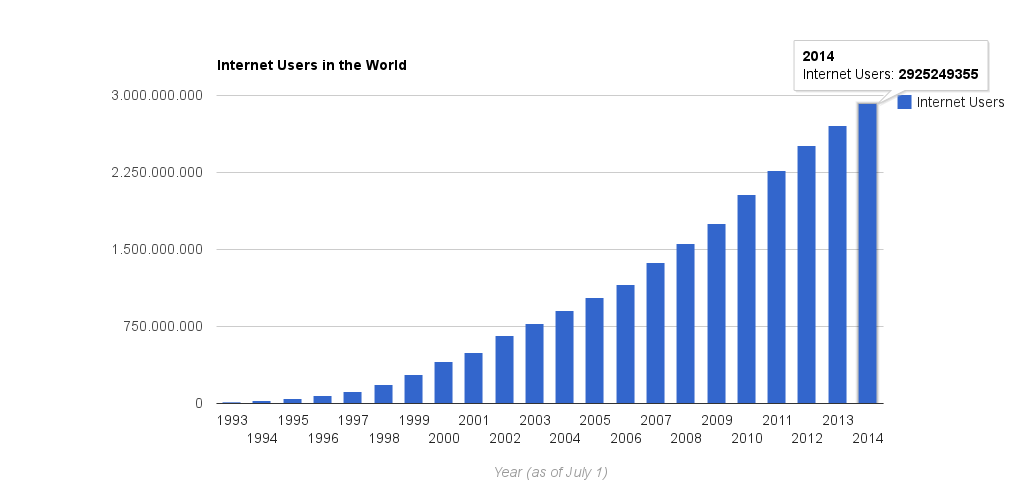
\includegraphics[scale=0.45]{images/internet_usage.png}
\caption{Quantidade de usuários da internet entre 1993 e 2014}
\label{fig:Quantidade de usuários da internet entre 1993 e 2014}
\end{figure}

\newpage

\item[Aplicações web] \hfill \\
A aplicação web refere-se a sistemas de informática que são executados através de navegadores com internet, geralmente aplicações que utilizam-se de tecnologias web como HTML, Javascript e CSS.\cite{appWeb}

Quando desenvolvemos uma aplicação web que visa atender a este aumento significativo de acessos, precisamos nos preocupar com a escalabilidade do sistema, sendo que escalabilidade vem a ser ``a habilidade de uma aplicação manter a performance\footnote{Que significa ``a habilidade que uma aplicação tem de atingir um objetivo, como por exemplo responder no menor tempo possível'' \cite{escTerm}} quando a carga de trabalho aumenta'' \cite{escTerm}, podendo ser considerada uma junção entre capacidade\footnote{Que significa ``a carga total que uma aplicação pode suportar''\cite{escTerm}} e performance. 


\item[Escalabilidade em aplicações web] \hfill \\
Existem duas formas de escalabilidades relacionadas as páginas web, a escalabilidade vertical, em que há uma melhoria do hardware de um único servidor, quando é adicionada mais memória, ou o processador é trocado por outro mais potente, entre outros aspectos, e a escalabilidade horizontal, que significa adicionar mais servidores, permitindo a criação de um \textit{cluster}\footnote{É um conjunto de computadores que subdividem o processamento do sistema para o aumento de desempenho, disponibilidade e balanceamento de carga.}. Estas duas formas de escalabilidade são relacionadas ao hardware, e são utilizadas por páginas web que tem uma grande quantidade de acessos, que precisam continuar respondendo as requisições de maneira satisfatória\footnote{Por exemplo sem que o usuário perceba atrasos no carregamento da página}.  

Existem  situações em que a aquisição ou o melhoramento de servidores se torna algo muito custoso ou até mesmo inviável, para estas situações são aplicadas técnicas de escalabilidade relacionadas ao software, que podemos subdividir em duas partes, que serão apresentadas a seguir:

\begin{itemize}
  \item A primeira é quando é realizado um simples acesso a página, ou seja, existem requisições do tipo \textit{http get}, neste caso para lidarmos com escalabilidade uma das soluções é a utilização de um proxy reverso\footnote{``Enquanto um Proxy, no modelo convencional, intercepta requisições originadas na rede local (LAN – Local Área Network) com destino à Internet, um Proxy Reverso intercepta requisições originadas na Internet com destino à rede local.'' \cite{proxyRev}}, que pode funcionar como uma cache para conteúdos estáticos\footnote{Musicas, imagens, vídeos, etc.} e dinâmicos\footnote{Que é quando um código é executado do lado do servidor para atender uma requisição, podendo realizar uma série de tarefas, como por exemplo acessar um banco de dados, sendo que este código é escrito em uma linguagem de programação como PHP, Java, Python, entre outras.}.

 \item A segunda parte é quando dados são enviados para serem persistidos através da página, neste caso estas requisições são do tipo \textit{http post}, sendo que não há como efetuar cache destes dados, pois são dados novos, e neste caso as soluções encontradas são desde enfileirar as entradas para o banco de dados, até a utilização de banco de dados NoSQL.
\end{itemize}

\end{description}

\section{Programação orientada a eventos}
\label{sec:Programação orientada a eventos}
\nocite{eventDrivenPro}
A programação orientada a eventos ou programação dirigida a eventos é considerada um paradigma da programação\footnote{Um paradigma de programação fornece e determina a visão que o programador possui sobre a estruturação e execução do programa.} e entender a orientação a eventos é importante para que se entenda algumas características do Node.JS. 

Entre outros paradigmas de programação podemos citar \cite{prdgProg}:
\begin{itemize}
  \item Imperativa: é um paradigma de programação que descreve a computação como ações, enunciados ou comandos que mudam o estado (variáveis) de um programa.
  \item Estruturada: é uma forma de programação de computadores que preconiza que todos os programas possíveis podem ser reduzidos a apenas três estruturas: sequência, decisão e iteração (esta última também é chamada de repetição).
  \item Orientada a objetos:é um modelo de análise, projeto e programação de sistemas de software baseado na composição e interação entre diversas unidades de software chamadas de objetos.
  \item Funcional: é um paradigma de programação que trata a computação como uma avaliação de funções matemáticas e que evita estados ou dados mutáveis. Ela enfatiza a aplicação de funções, em contraste da programação imperativa, que enfatiza mudanças no estado do programa.
\end{itemize}

Um evento é qualquer ação do usuário que interaja com o sistema, por exemplo um clique do mouse em determinado local da aplicação, teclas do teclado sendo pressionadas ou até mesmo um toque na tela, caso o hardware permita como em smartphones e tablets modernos.

Um programa que utiliza orientação a eventos possui um fluxo que é um laço que recebe repetidamente informação para processar e disparam uma função de resposta de acordo com o evento recebido. As informações de entrada podem ser enfileiradas ou registrar uma interrupção, em alguns casos ambos podem ser adotados. Diferentemente do fluxo de linguagens tradicionais como C, que o fluxo é linear com loops no decorrer do caminho.

Para facilitar o entendimento imagine uma aplicação que mostra em sua tela o número zero, e esse numero é incrementado ao se pressionar o botão esquerdo do mouse, e decrementado caso o botão direito seja pressionado, e o número volta para zero quando for pressionado o botão do meio. Esses cliques representam eventos e quando ocorrem, o sinal destes eventos são passados ao event loop que os trata e retorna o resultado, neste caso o retorno é o incremento, decremento ou resetar o valor.

A figura \ref{fig:event loop} mostra como esse processo ocorre, destacando a interação dos eventos com o \textit{Event Loop}.

\begin{figure}[htb]
\centering
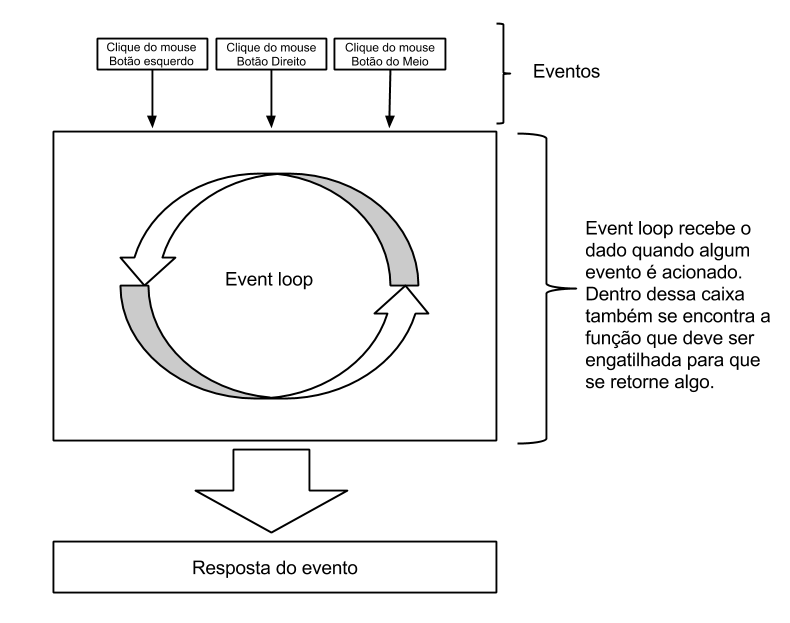
\includegraphics[scale=0.6]{images/event_loop_diagram.png}
\caption{Event Loop}
\label{fig:event loop}
\end{figure}

\newpage

\section{Javascript}
\label{sec: Javascript}
O Javascript  é uma linguagem de programação interpretada, que foi criada com o intuito de ajudar os navegadores web a executar scripts no lado do cliente e assim permitir a interação com o usuário\nocite{jsGood}. Esta linguagem foi baseada na ECMAScript\footnote{Que  é uma linguagem de programação de scripts.} que é padronizada pela Ecma international nas especificacões ECMA-262\footnote{\url{http://www.ecma-international.org/publications/files/ECMA-ST/Ecma-262.pdf}} e ISO/IEC 16262\footnote{\url{http://www.iso.org/iso/home/store/catalogue_tc/catalogue_detail.htm?csnumber=55755}}. Abaixo serão descritas algumas das parincipais caracteristicas do Javascript:

\begin{description}
\item[Imperativa e estruturada] \hfill \\ 
O Javascript possui elementos de sintaxe de linguagens de programação estruturada, elementos que se assemelham por exemplo com a linguagem C como \textit{If}, \textit{while} e \textit{switch}.

Apesar de sintaticamente parecer com C, seu escopo é diferente, Javascript utiliza-se de um escopo á nível de função\footnote{Isso significa que somente funções podem criar novos escopos, blocos como \textit{if}, \textit{while}, \textit{for} não criam novos escopos.}.

\item[Tipagem dinâmica] \hfill \\
No Javascript os tipos são associados com valores e não com as variáveis. Por exemplo, uma variável ``A'' poderia ser associado a um número e posteriormente ser associado a uma string. 

% \item[Baseada em objetos] \hfill \\
% A linguagem Javascript possui suporte a  objetos, que são implementados como listas associativas. Os nomes das propriedades de um objeto  são strings e podem, junto com seus valores, ser adicionadas, mudadas ou apagada em tempo de execução. Vale ressaltar que em Javascript existem alguns objetos padrões como \textit{window} e \textit{document}.

\item[Baseada em protótipos] \hfill \\
 O Javascript utiliza-se de protótipos no lugar das classes para o mecanismo de herança. É possível simular muitas características de orientação a objetos usando-se de protótipos.

\item[Linguagem orientada a eventos] \hfill \\
 No Javascript é possível tratar as interações do usuário em um arquivo HTML, e é através de eventos que isso é feito, como explicado na seção \ref{sec:Programação orientada a eventos} deste capítulo .

\end{description}

\section{NoSQL - Not Only SQL}
\label{sec: NoSQL - Not Only SQL}
Os banco de dados relacionais não foram desenvolvidos para resolver problemas enfrentados pelas aplicações web modernas como a escalabilidade e a agilidade \cite{mongoNosql}, pois ``foram projetados para serem executados em uma máquina apenas'' \cite{compBds}, sendo que ``quanto maior o tamanho, mais custoso se torna essa escalabilidade, seja pelo custo de novas máquinas, seja pelo aumento de especialistas nos bancos de dados utilizados''.\cite{IntNosql}

Devido as limitações citadas começaram surgir diversas soluções que funcionam de maneira diferente aos tradicionais banco de dados relacionais, essas soluções ficaram conhecidas como NoSQL, que é uma sigla que significa \textit{Not Only SQL}, e que podemos descrever como ``uma nova classe de banco de dados'' \cite{AnaliseNosql} formada por ``diferentes sistemas de armazenamento ''\cite{NosqlIm} que surgiram para lidar nas situações em que os banco de dados tradicionais são ineficientes .``Muitas dessas bases apresentam características muito interessantes como alta performance, escalabilidade, replicação, suporte à dados estruturados e sub colunas''\cite{NosqlIm}. 

Segue abaixo algumas características de bancos de dados NoSQL\cite{compBds}:
\begin{itemize}
\item Não usa modelo de dados relacional e portanto não usa a linguagem SQL;
\item Costuma ser projetado para ser executado em um \textit{cluster};
\item Costuma ser \textit{Open-Source};
\item Não possui esquema fixo (\textit{SCHEMA-LESS}), permitindo gravar qualquer dado em qualquer estrutura.
\end{itemize}

Exitem diversas categorias\cite{NosqlDatabase} em que podemos classificar os banco de dados NoSQL que variam de acordo com a forma de armazenar os dados. Algumas das  principais categorias que podemos destacar são: chave/valor, orientado a colunas, orientado a documentos e baseado em grafos \cite{AnaliseNosql}.
\begin{description}
\item[Chave/Valor] \hfill \\ 
Utiliza um array associativo como modelo de dados \cite{NosqlWiki}, sendo que neste array os dados podem ser acessados através de chaves, e estas chaves estão associadas a seus valores correspondentes. Alguns bancos desta categoria são Azure Table Storage, Berkeley DB,Couchbase, DynamoDB, Redis, Riak e Tokyo Cabinet.

%exemplos
\item[Orientado a colunas] \hfill \\ 
Em um banco de dados orientado a colunas ´´ao invés de cada registro da tabela ficar armazenado em uma linha, o registro passa a ser armazenado em colunas separadas.''\cite{NosqlCol}. Como exemplo de banco de dados desta categoria temos:  Hadoop, Cassanda, Hypertable e Amazon SimpleDB.

% Essa forma de armazenamento tem algumas vantagens, como exemplo a capacidade de compressão dos dados, se formos analisar a compressão de um banco onde os registros são armazenados em linha, encontraremos em uma mesma linha diferentes tipos (domínios) o que torna o processo mais complicado, já no banco orientado a colunas, cada coluna irá conter o mesmo tipo (domínio) de dado. De acordo com algumas pesquisas o nível de compressão alcançado  em bancos orientados a colunas chega a ser de 60% a 70%  mais eficiente que nos bancos orientados a linhas.
\item[Orientado a documentos] \hfill \\ 
Nesta categoria de banco de dados o armazenamento é realizado através de documentos, e o conjuntos de documentos formam uma coleção. Geralmente os documentos são codificados nos formatos JSON, XML e YAML\cite{NosqlWiki}. Alguns dos bancos de dados que pertencem a esta categoria são: MongoDB, CouchDB e EjDB.


\item[Baseado em grafos] \hfill \\ 
Quando temos dados cujas relações são bem representadas como um grafo, podemos utilizar um banco de dados baseado em grafos \cite{NosqlWiki}. Com este modelo podemos ``representar os dados e/ou o esquema dos dados como grafos dirigidos, ou como estruturas que generalizem a noção de grafos.'' \cite{IntNosql}

Alguns bancos que fazem parte desta categoria são: Neo4J, Infinite Graph, Titan, e Bigdata.

\end{description}

%\section{Vantagens da utilização do MEAN para o desenvolvimento de aplicações escaláveis}

